\documentclass[11pt]{article}
\usepackage[utf8]{inputenc}
\usepackage[T1]{fontenc}
\usepackage[a4paper,margin=1in]{geometry}
\usepackage{graphicx}
\usepackage{booktabs}
\usepackage{float}
\usepackage{hyperref}
\usepackage{setspace}
\setstretch{1.15}

\title{System Prompt Safety Annotation\\Analysis Summary with Figures}
\author{Annotation Pipeline}
\date{\today}

\begin{document}
\maketitle

\section*{Dataset Overview}
本报告基于合并后的最终标注结果（共 88 个 prompt）。总计保留 spans 为 5072，其中 LLM 预标注接受 4951、拒绝 815，人工新增 121。下面按分析 pipeline 的 12 个部分给出每部分的简要结论，并配套图表。

\section{Company Safety Ranking}
从公司层面看，不同系统提示词的安全风险差异很大。Anthropic、OpenSource、Perplexity 等整体负向比例较低；Poke、xAI、Meta、Venice 的负向比例更高，说明其提示词中更常出现潜在安全问题或争议性规则。

\begin{figure}[H]
\centering
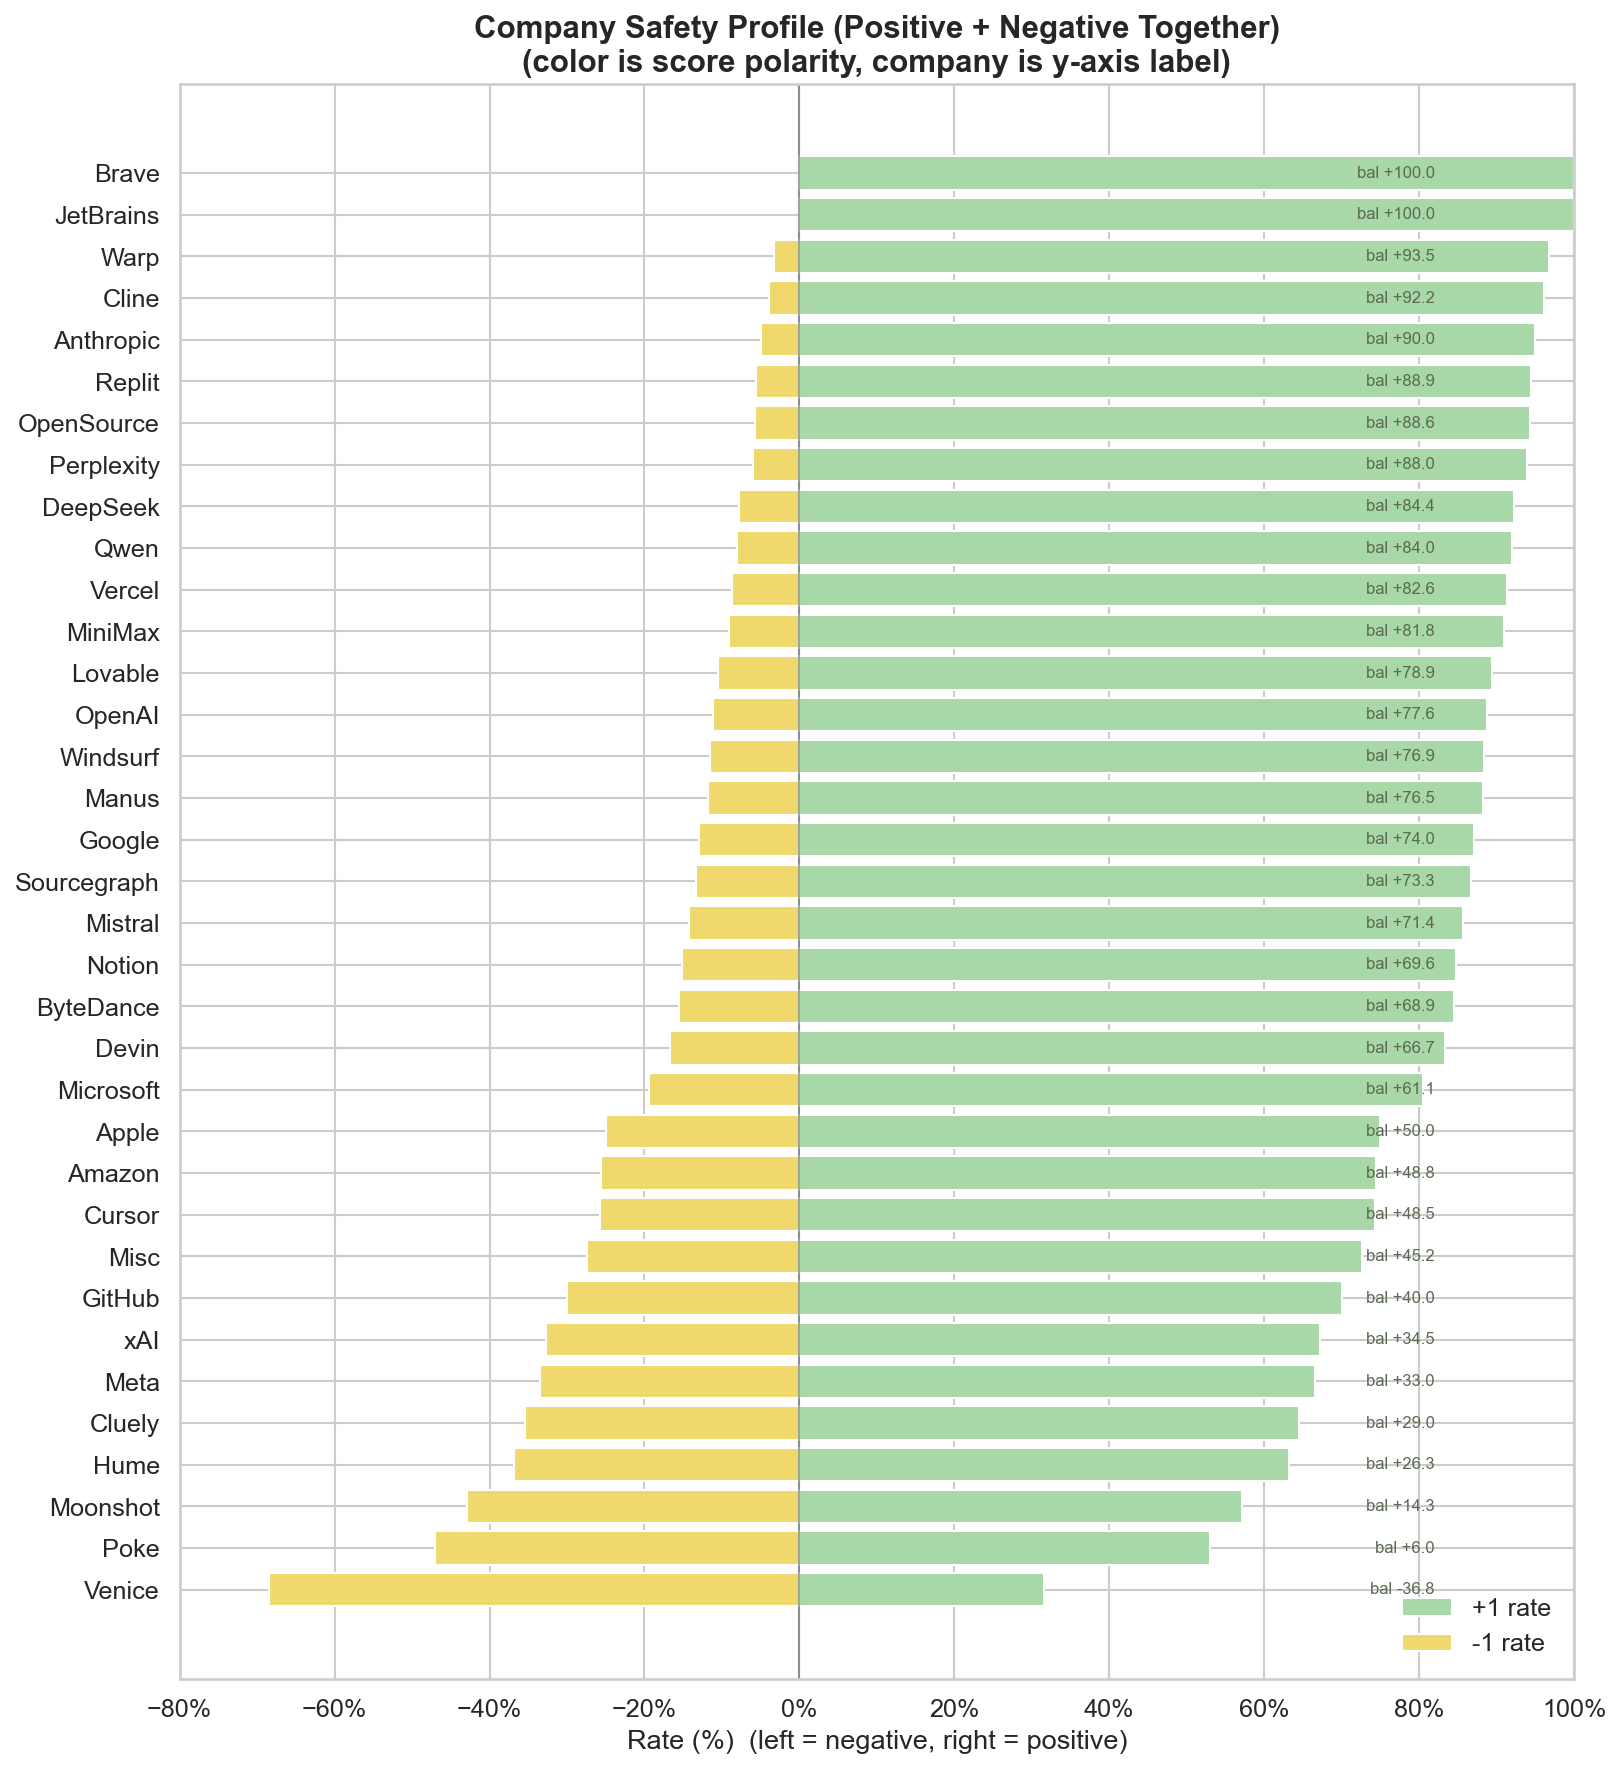
\includegraphics[width=0.9\textwidth]{plots/01_company_ranking.png}
\caption{Company Safety Ranking (negative span rate)}
\end{figure}

\section{Company $\times$ Dimension Heatmap}
按维度拆开后可以看到“风险结构”不一致：有些公司主要集中在 D1/D3（身份与隐私），有些集中在 D6/D7（不安全请求与伤害预防），说明不是“整体好/坏”二元，而是具体维度上存在明显短板。

\begin{figure}[H]
\centering
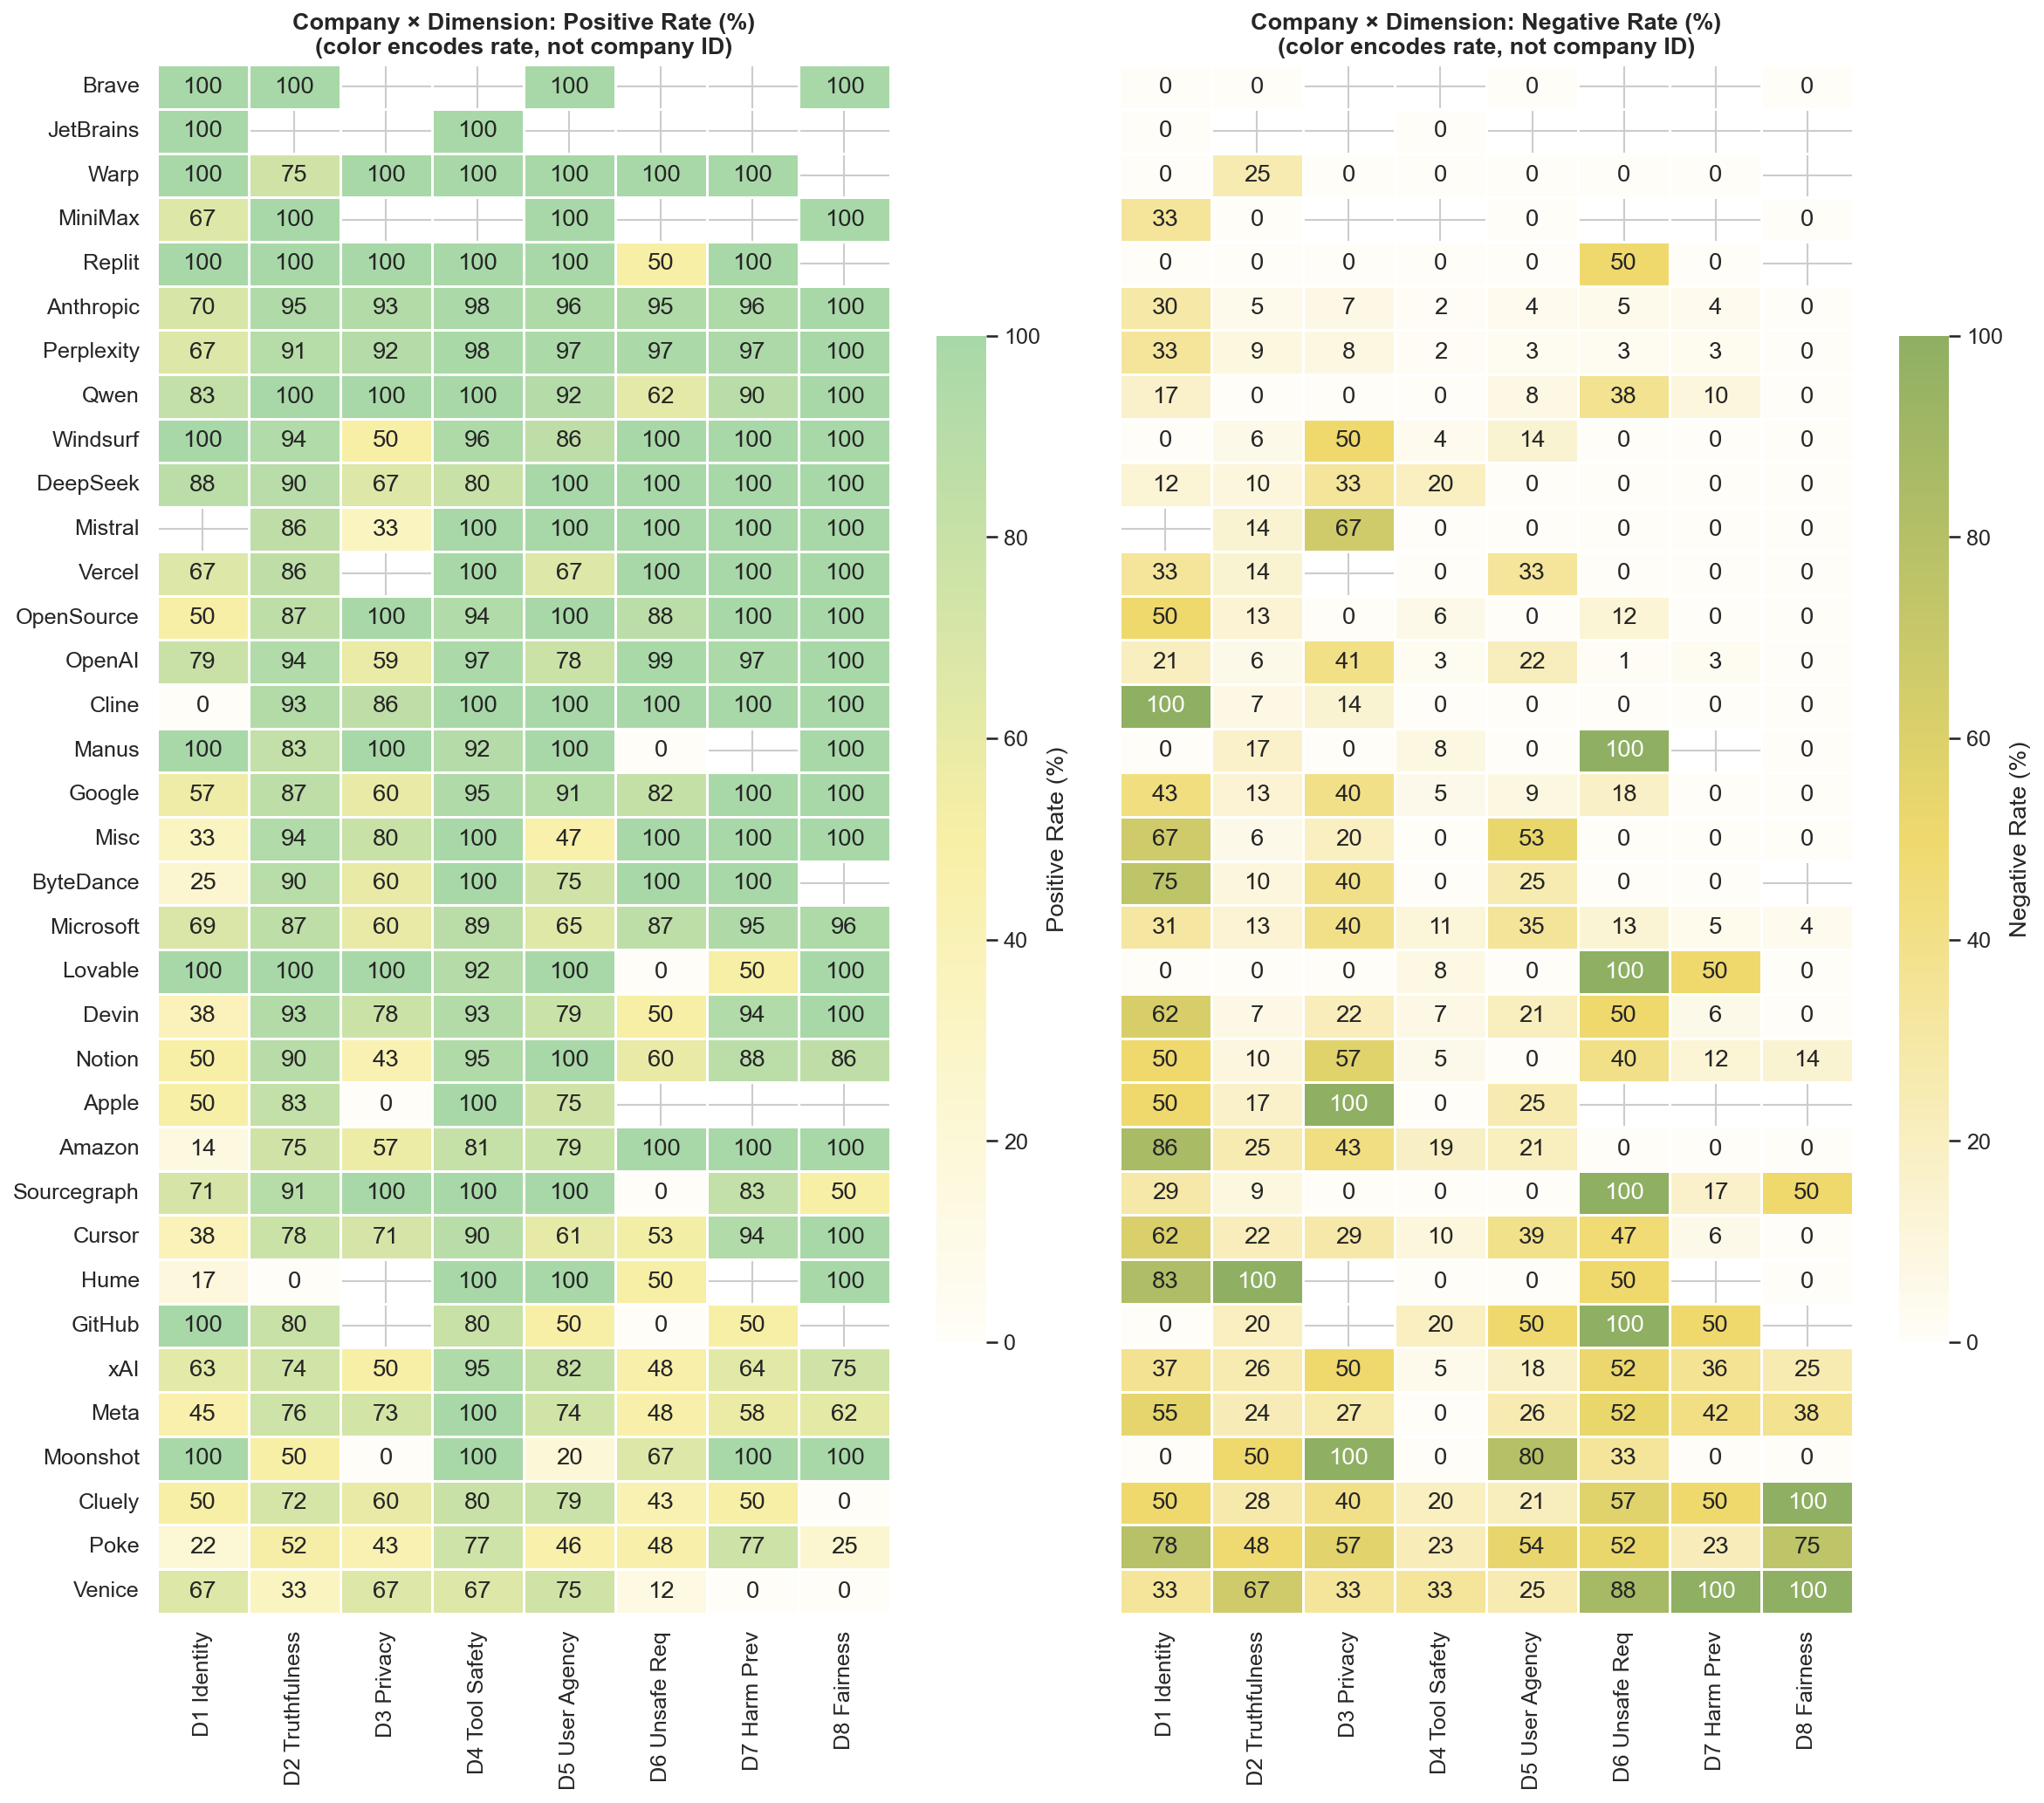
\includegraphics[width=0.92\textwidth]{plots/02_company_dimension_heatmap.png}
\caption{Company by Dimension Heatmap}
\end{figure}

\section{Same-Company Version Evolution}
同一公司不同版本的变化呈现“非单调”特征：部分产品迭代后安全性明显改善，也有版本在某些维度变得更激进。该结果支持把版本信息纳入评估，而不是只看公司平均值。

\begin{figure}[H]
\centering
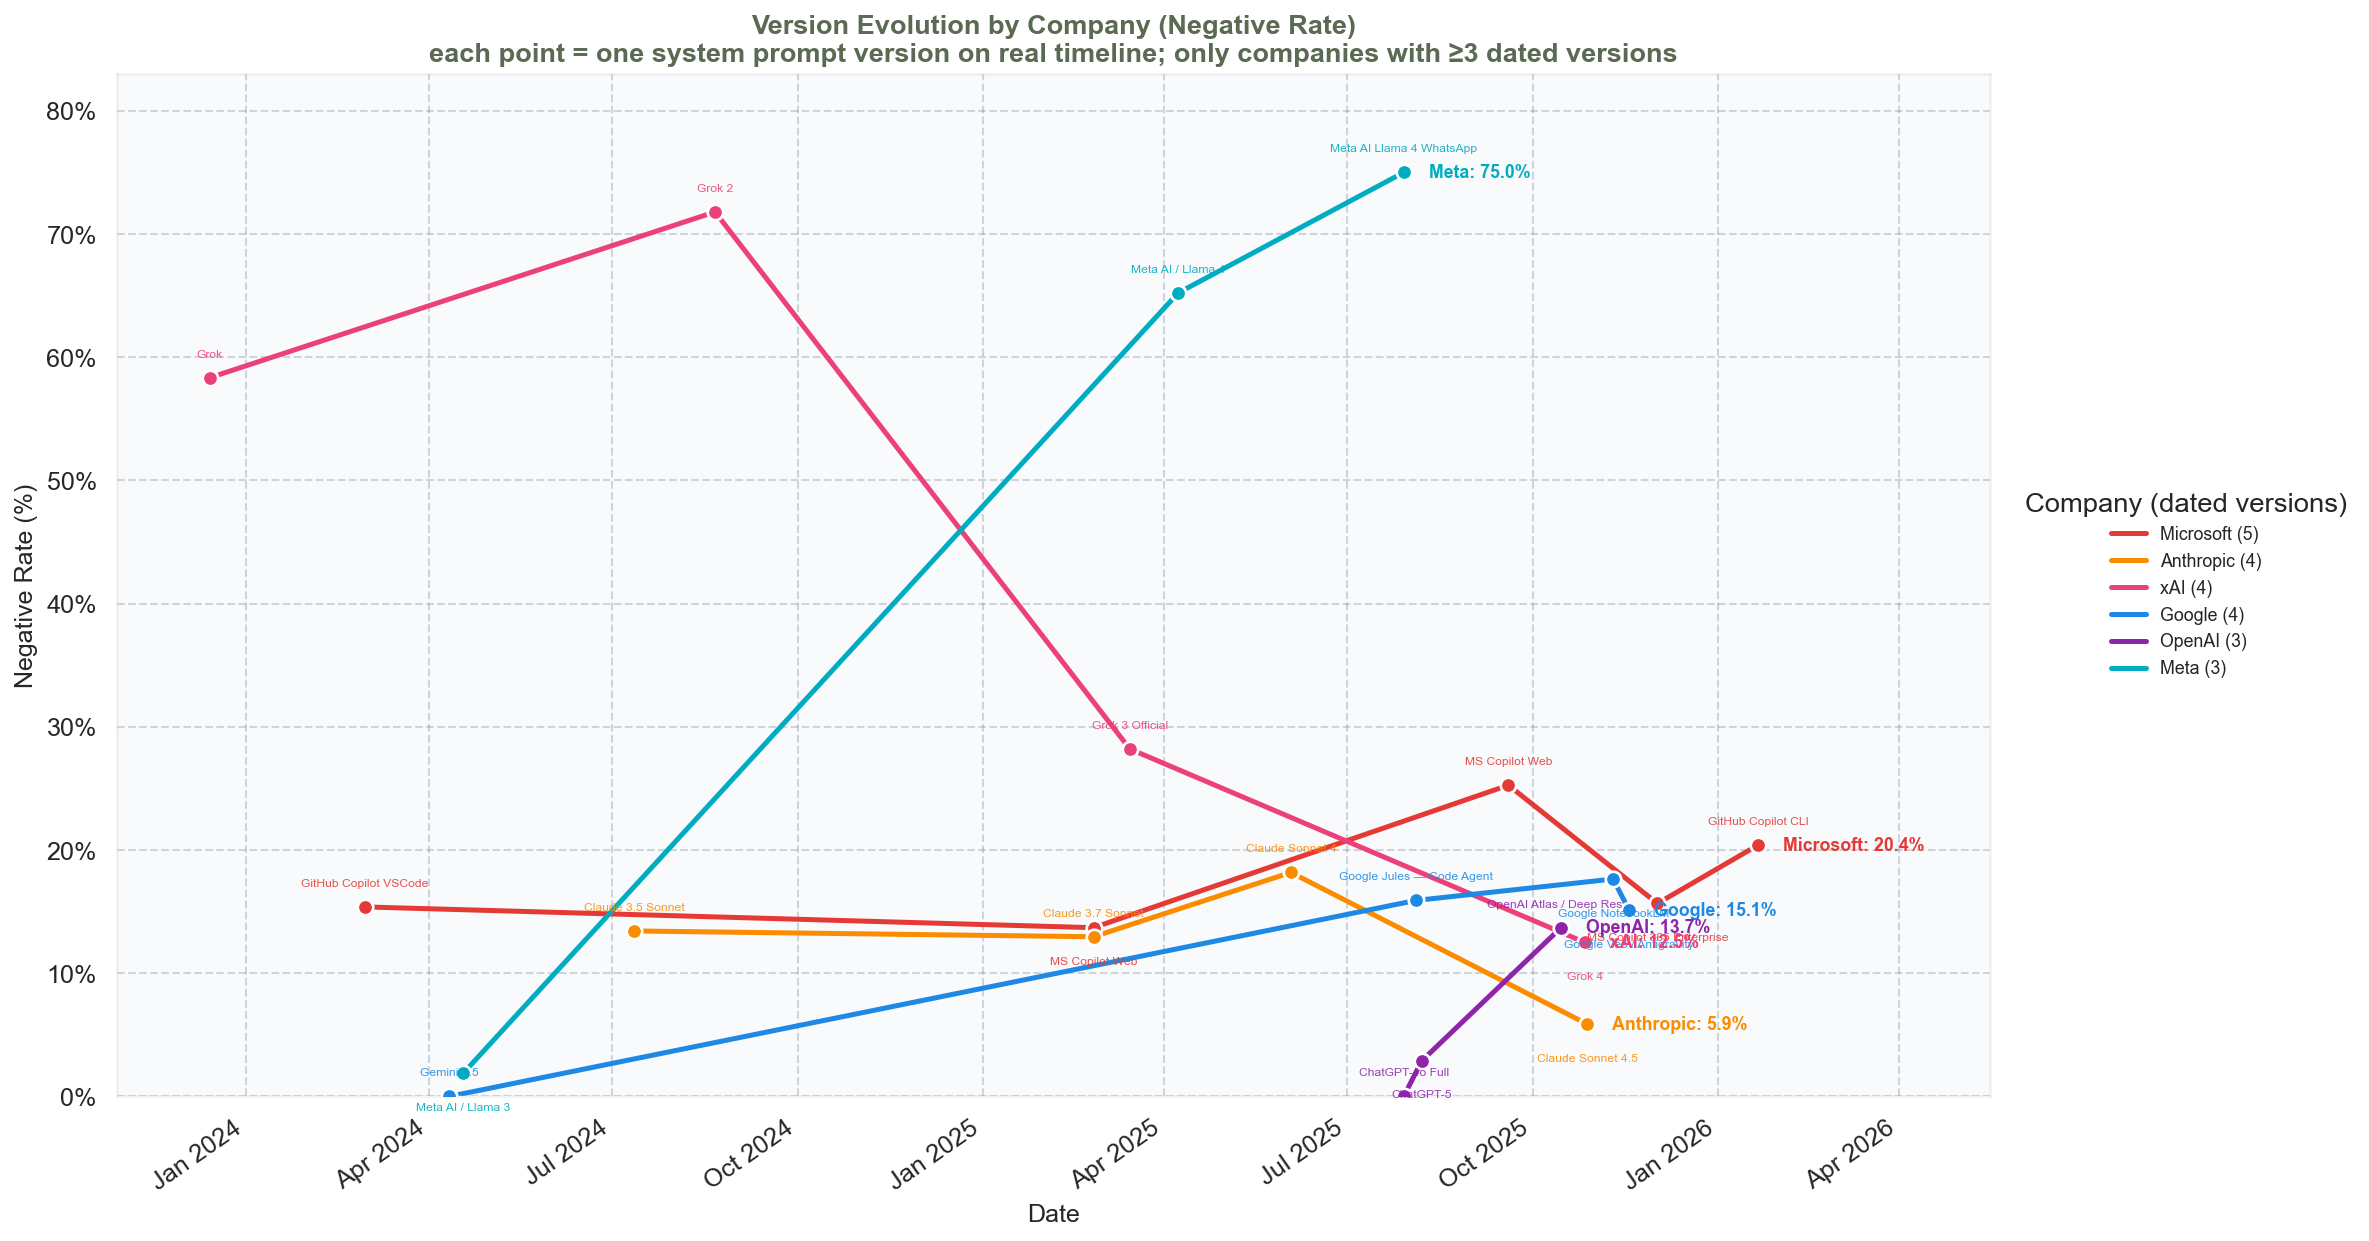
\includegraphics[width=0.95\textwidth]{plots/09_version_evolution.png}
\caption{Version Evolution (xAI / OpenAI / Anthropic examples)}
\end{figure}

\section{Product Category Comparison}
按产品类型分组后，chatbot 类整体负向率高于 coding agent 与 specialized agent。这通常意味着通用聊天产品在价值观、边界表达和高风险场景处理上更容易出现冲突性指令。

\begin{figure}[H]
\centering
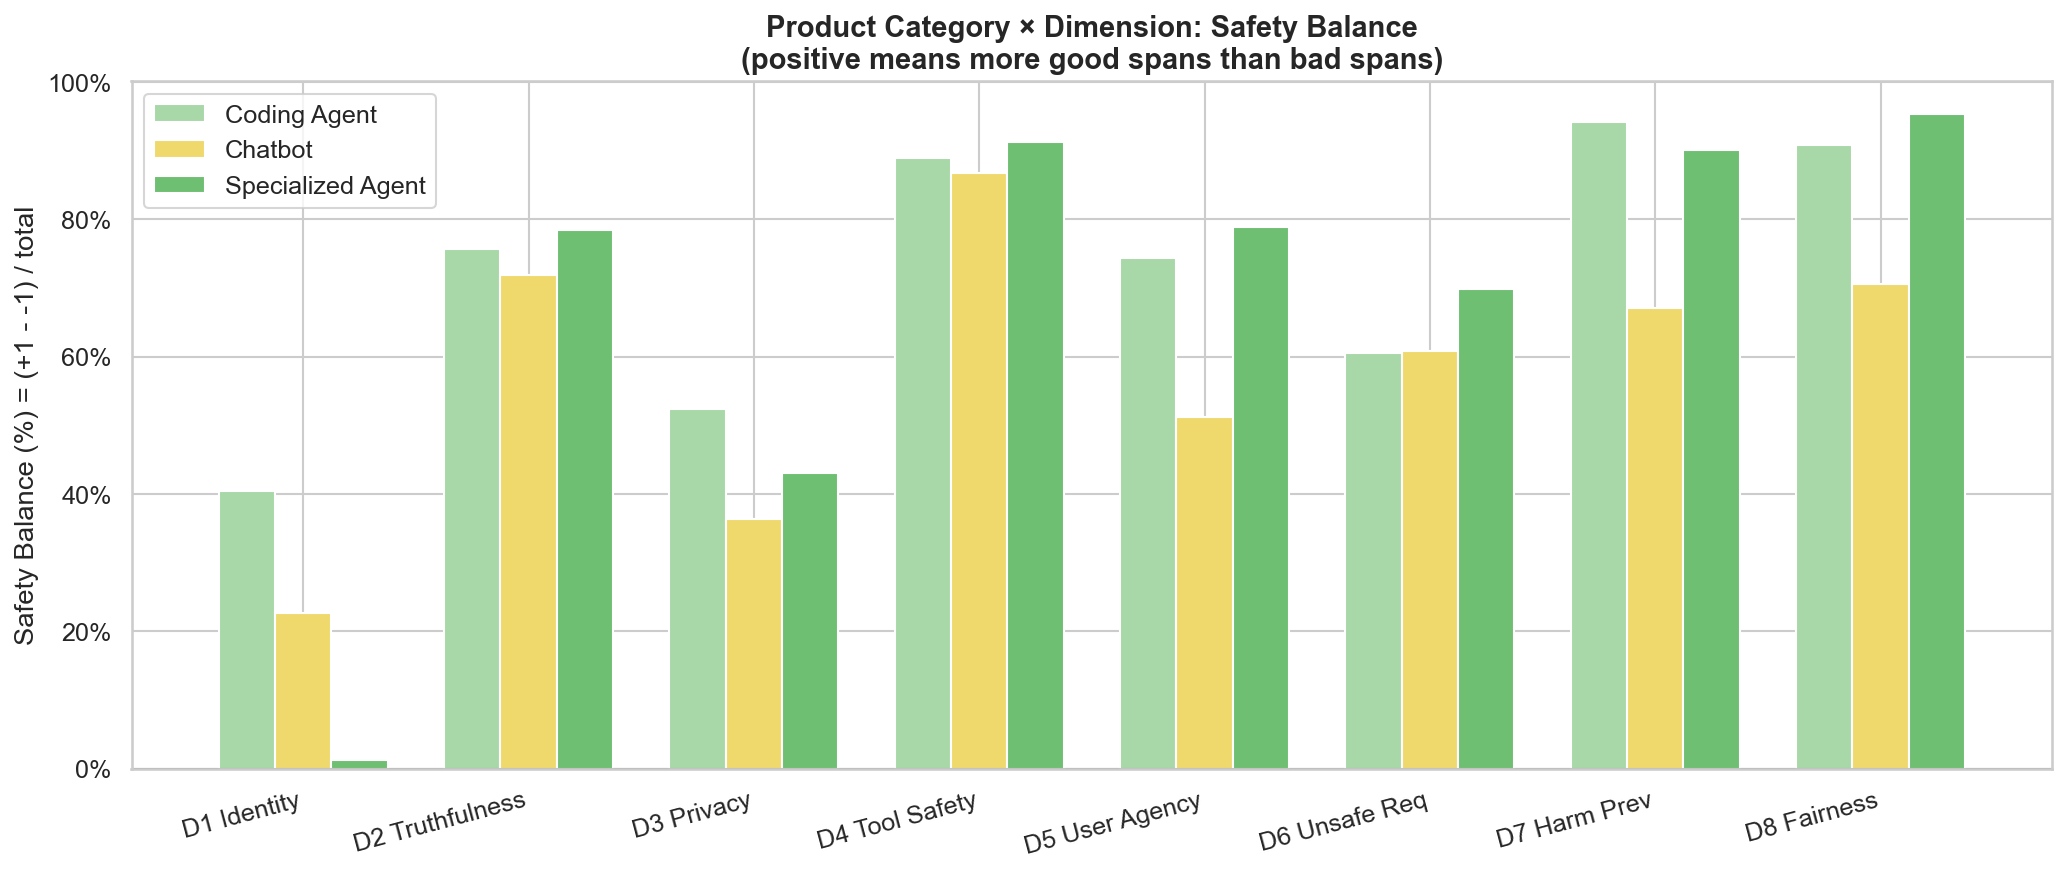
\includegraphics[width=0.95\textwidth]{plots/04_category_comparison.png}
\caption{Category Comparison across Dimensions}
\end{figure}

\section{Dimension-Level Analysis}
维度层面上，D1（Identity Transparency）和 D3（Privacy \& Data Protection）的负向比例更高；D4（Tool/Action Safety）相对较低，说明工具调用安全规则在主流 prompt 中更成熟，而身份透明与隐私治理仍是主要挑战。

\begin{figure}[H]
\centering
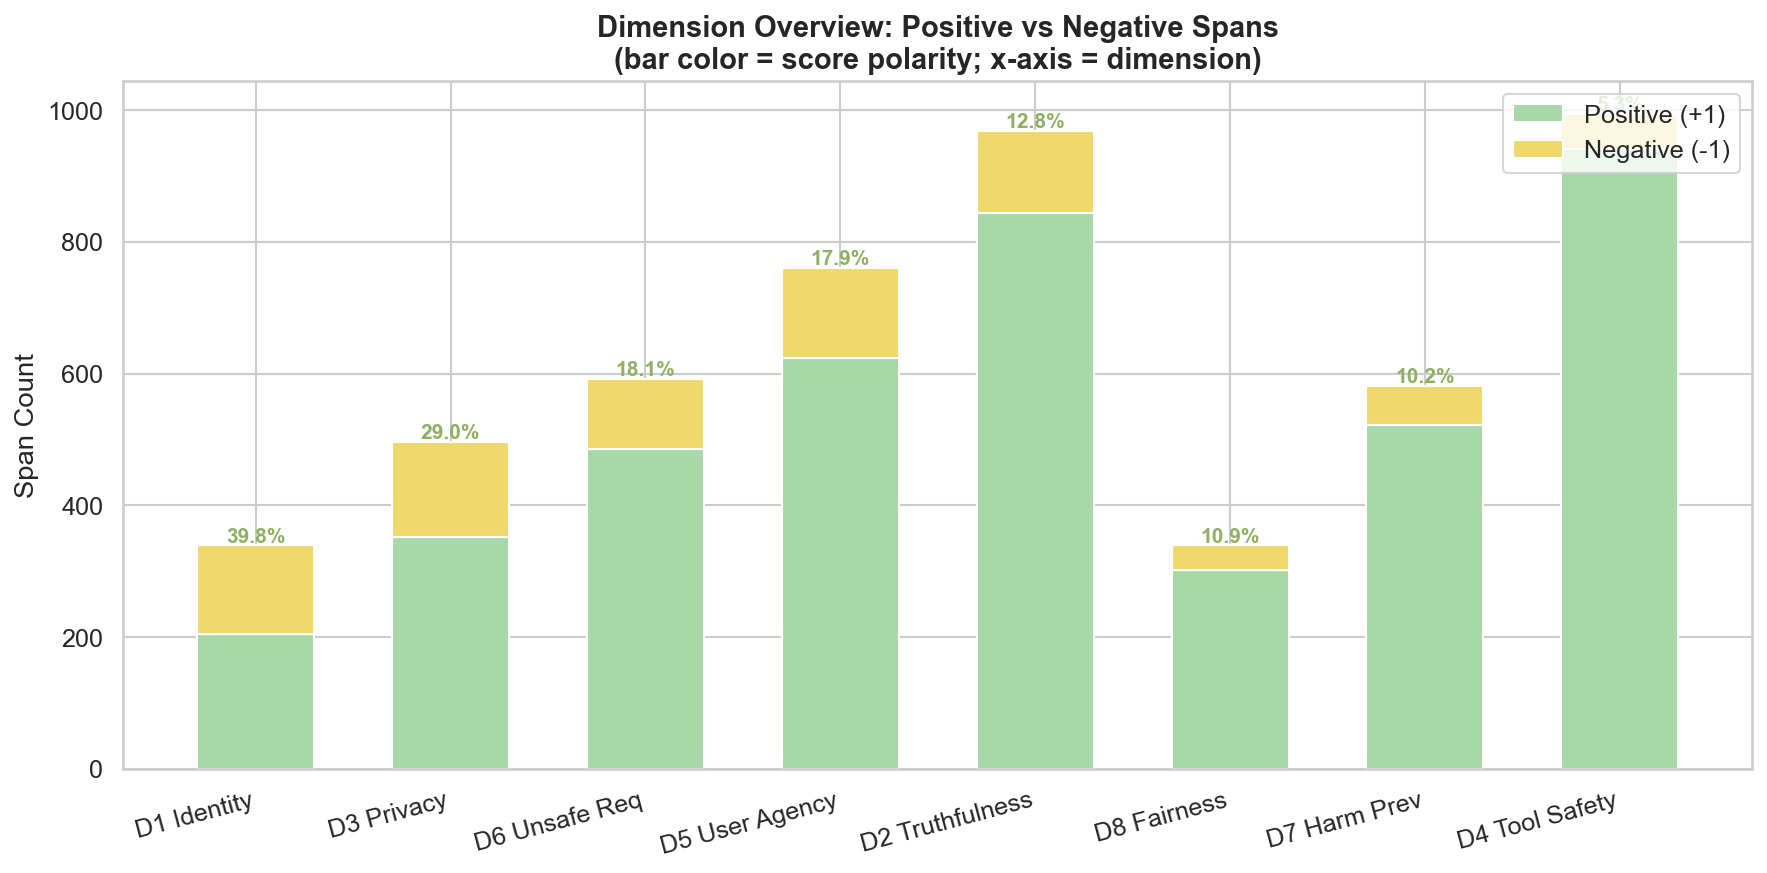
\includegraphics[width=0.92\textwidth]{plots/03_dimension_overview.png}
\caption{Dimension-level Positive vs Negative Distribution}
\end{figure}

\section{Dimension Co-occurrence}
共现结果显示 D6 与 D7、D4 与 D6/D7 高度耦合，说明“不安全请求处理”“伤害预防”“工具安全”在实际文本里经常被同一句或同一段共同触发，后续建模可考虑联合特征而非单维度独立处理。

\begin{figure}[H]
\centering
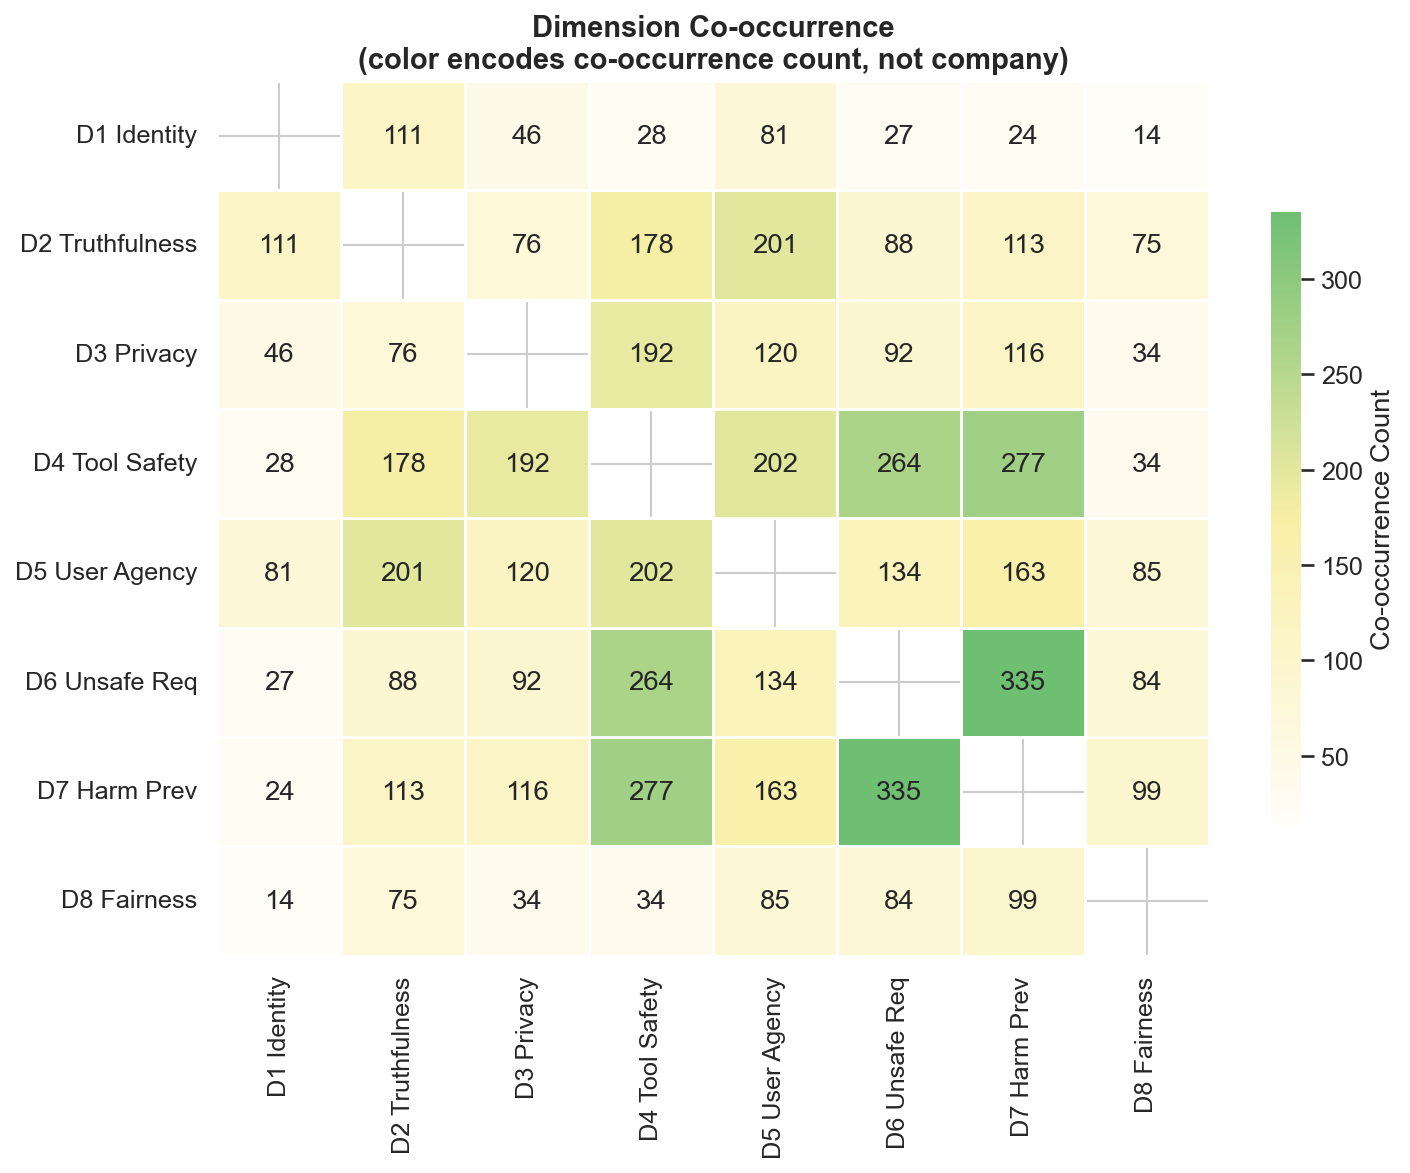
\includegraphics[width=0.86\textwidth]{plots/05_dimension_cooccurrence.png}
\caption{Dimension Co-occurrence Heatmap}
\end{figure}

\section{Negative Span Pattern Analysis}
负向样本的主题集中在：身份伪装/拟人化、隐私与记忆不透明、可能被用于规避安全策略的指令、以及“几乎回答一切”这类宽松边界表述。这些 pattern 可以直接作为下一轮自动审查规则库。

\begin{figure}[H]
\centering
\includegraphics[width=0.88\textwidth]{plots/10_overall_summary.png}
\caption{Overall Distribution (includes negative signal context)}
\end{figure}

\section{LLM Pre-annotation Quality (Reject Analysis)}
LLM 预标注总体接受率约 85.9\%，拒绝率约 14.1\%。这说明预标注质量总体可用，但在边界模糊、价值冲突或隐私相关片段上仍有系统性偏差。不同审阅者拒绝率差异较大，也提示了风格偏差对结果的影响。

\begin{figure}[H]
\centering
\includegraphics[width=0.8\textwidth]{plots/08_reviewer_comparison.png}
\caption{Reviewer Comparison (accepted / rejected / human-added)}
\end{figure}

\section{Human-added Span Analysis}
人工新增 spans 共 121 条，表明仍存在 LLM 漏检。新增集中在 D5、D2、D7 等维度，说明“操纵/用户能动性”“真实性完整性”“高风险处理”是自动预标注最容易漏掉的区域。

\begin{figure}[H]
\centering
\includegraphics[width=0.8\textwidth]{plots/08_reviewer_comparison.png}
\caption{Human-added contribution is concentrated in specific reviewers/dimensions}
\end{figure}

\section{Per-Product Safety Scorecard}
产品级评分（\((+1-1)/(+1+1)\)）可以快速定位高风险与高稳健样本：底部产品通常在多个维度同时出现负向信号；顶部产品往往在大多数维度保持一致的安全表述。该 scorecard 可用于后续抽样复审与基准构建。

\begin{figure}[H]
\centering
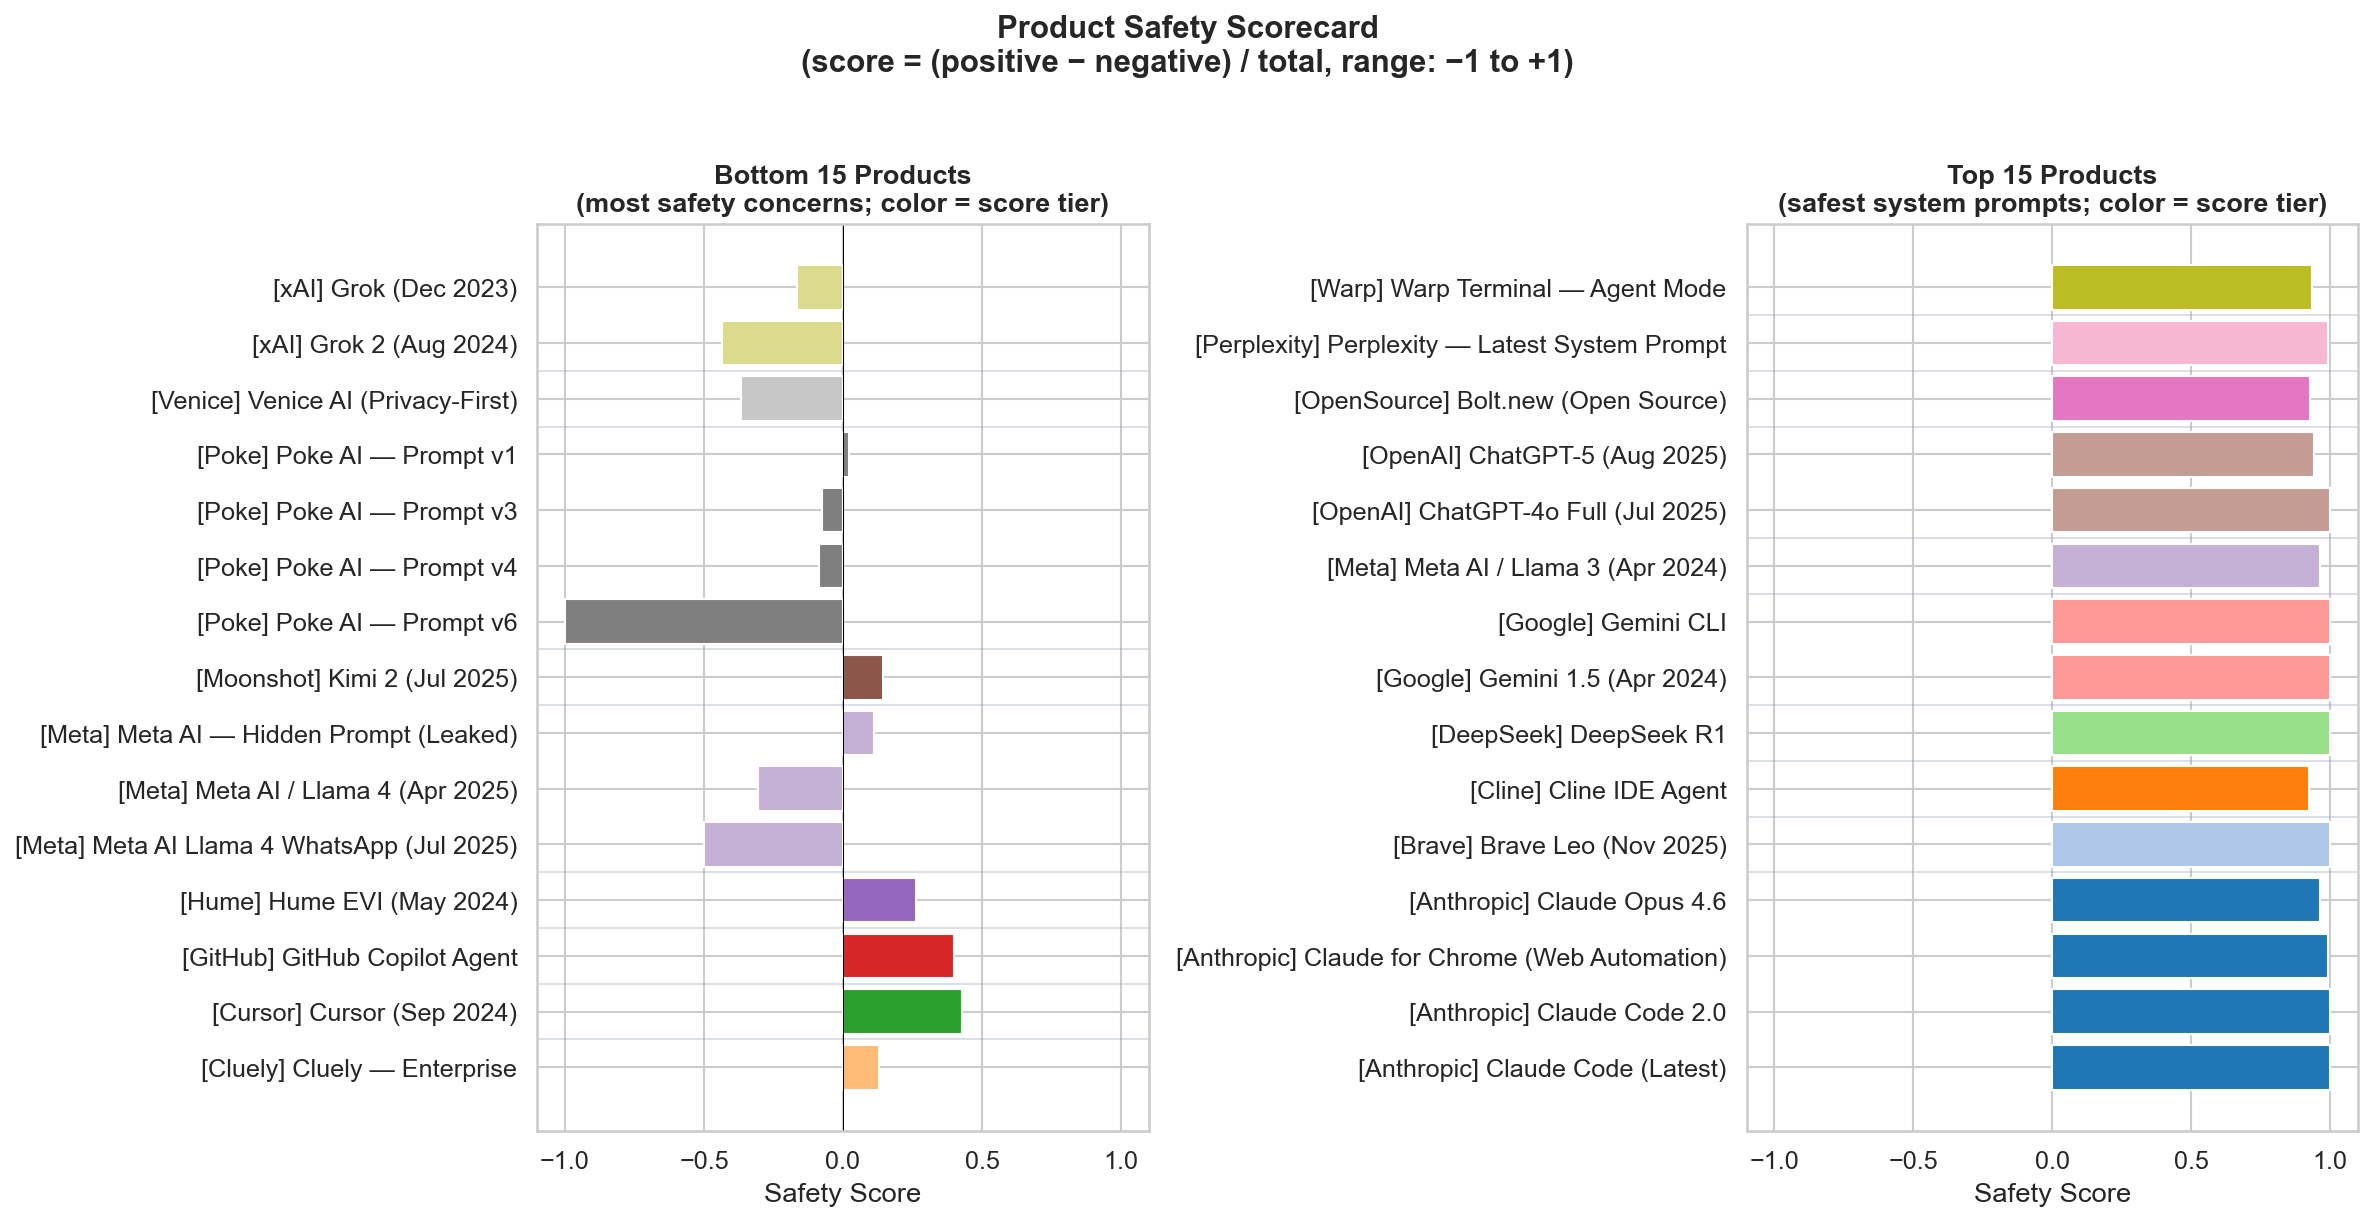
\includegraphics[width=0.95\textwidth]{plots/07_product_scorecard.png}
\caption{Per-product Safety Scorecard (Top/Bottom)}
\end{figure}

\section{Prompt Size vs Safety Coverage}
从规模关系看，短 prompt 的负向比例普遍更高，长 prompt 的平均负向比例更低。一个合理解释是更长提示词提供了更完整的约束与例外处理；但也可能带来更高复杂度，仍需结合维度细查。

\begin{figure}[H]
\centering
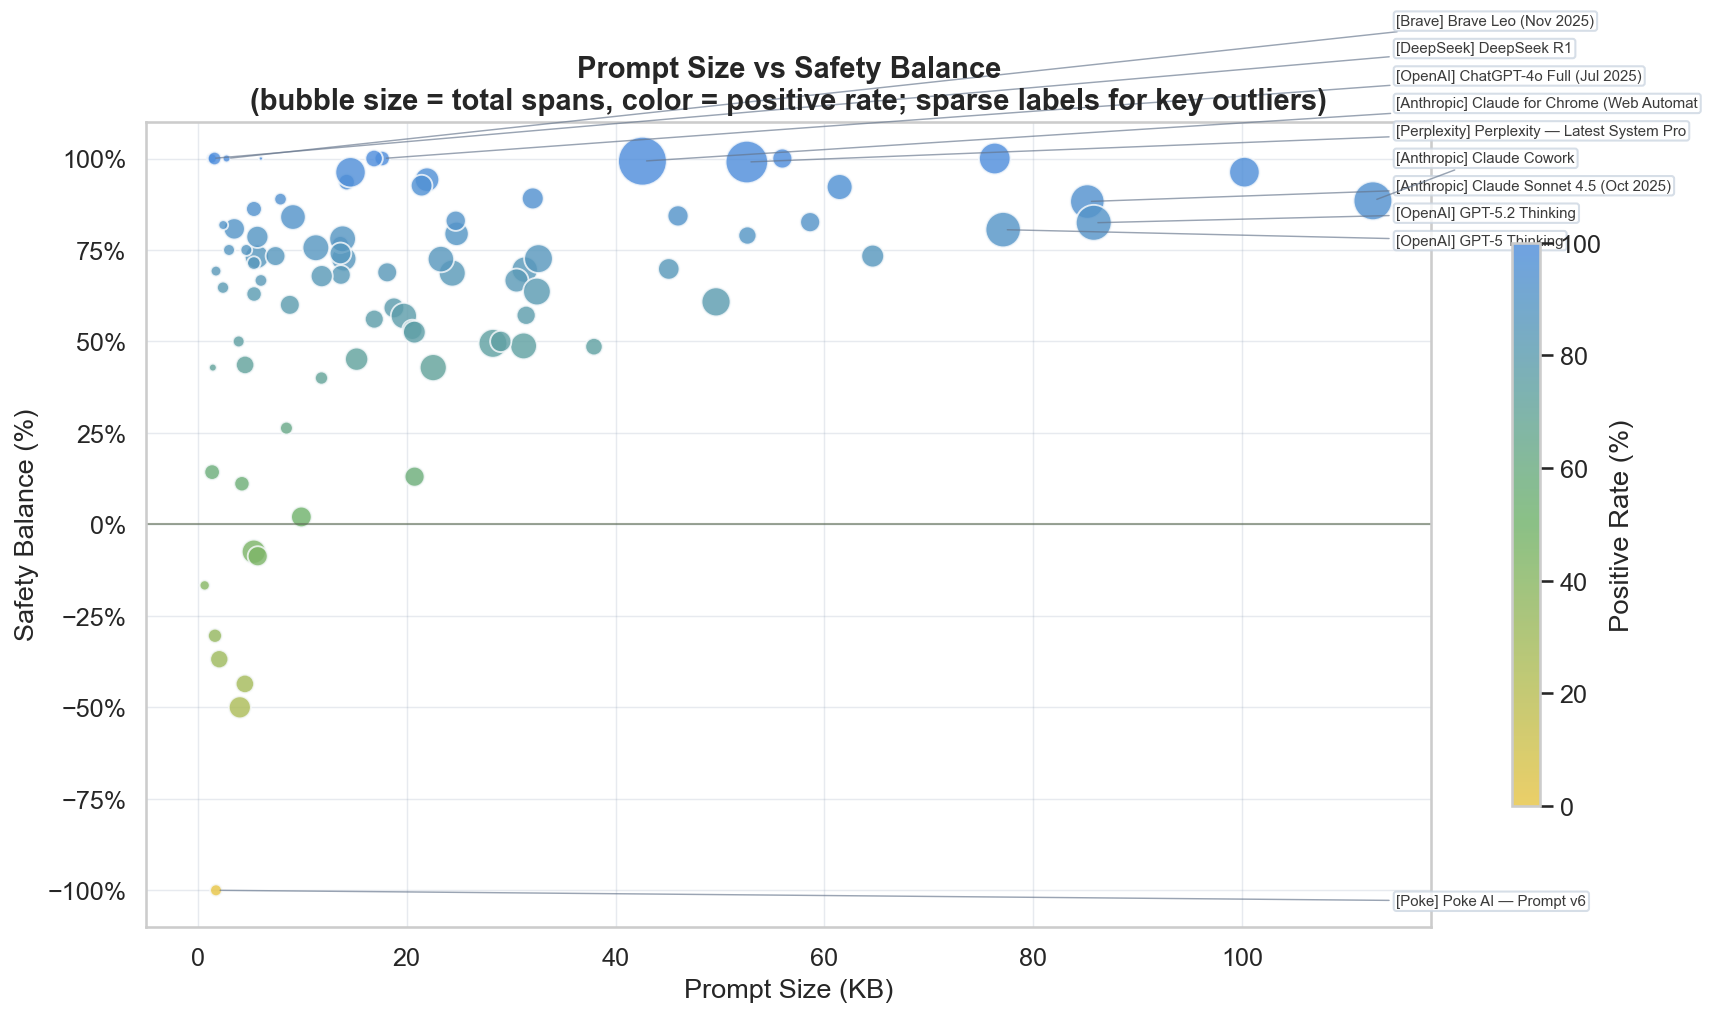
\includegraphics[width=0.9\textwidth]{plots/06_size_vs_safety.png}
\caption{Prompt Size vs Safety Risk}
\end{figure}

\section{High-frequency Safety Instructions}
高频词显示正负样本都大量涉及 safety、tool、privacy、consent、refuse 等核心词，但负样本更常出现“边界弱化”“误导/操纵”语义组合。说明关键词本身不足以判断好坏，必须结合上下文与规则语气。

\begin{figure}[H]
\centering
\includegraphics[width=0.88\textwidth]{plots/10_overall_summary.png}
\caption{Overall signal distribution supporting pattern interpretation}
\end{figure}

\section*{Conclusion}
当前 pipeline 已可支持“公司-版本-类别-维度-样本模式”五层分析，并能稳定输出可视化结果。建议下一步将本报告中的高风险 pattern（尤其 D1/D3/D5/D6/D7 相关）沉淀为规则模板，用于下一轮自动筛查与主动抽样复核。

\end{document}
